\documentclass[tikz, border=10pt]{standalone}
\usepackage{tikz}
\usetikzlibrary{shapes.geometric, arrows.meta, positioning, fit, calc}

\tikzset{
  proc/.style={
    rectangle, rounded corners=4pt,
    draw=black!70, fill=blue!8,
    text width=5.2cm, align=center,
    minimum height=0.75cm,
    font=\small\ttfamily
  },
  opt/.style={
    rectangle, rounded corners=4pt,
    draw=blue!60, fill=blue!4,
    text width=3cm, align=center,
    minimum height=0.7cm,
    font=\small,
    dashed
  },
  file/.style={
    rectangle, rounded corners=2pt,
    draw=teal!70, fill=teal!10,
    text width=5.2cm, align=center,
    minimum height=1cm,
    font=\small\ttfamily
  },
  side/.style={
    rectangle, rounded corners=4pt,
    draw=orange!70, fill=orange!8,
    text width=3.8cm, align=center,
    minimum height=0.75cm,
    font=\small\ttfamily
  },
  arr/.style={-{Stealth[length=6pt]}, thick, black!70},
  darr/.style={-{Stealth[length=6pt]}, thick, blue!50, dashed},
  lbl/.style={font=\footnotesize, midway, fill=white, inner sep=2pt}
}

\begin{document}
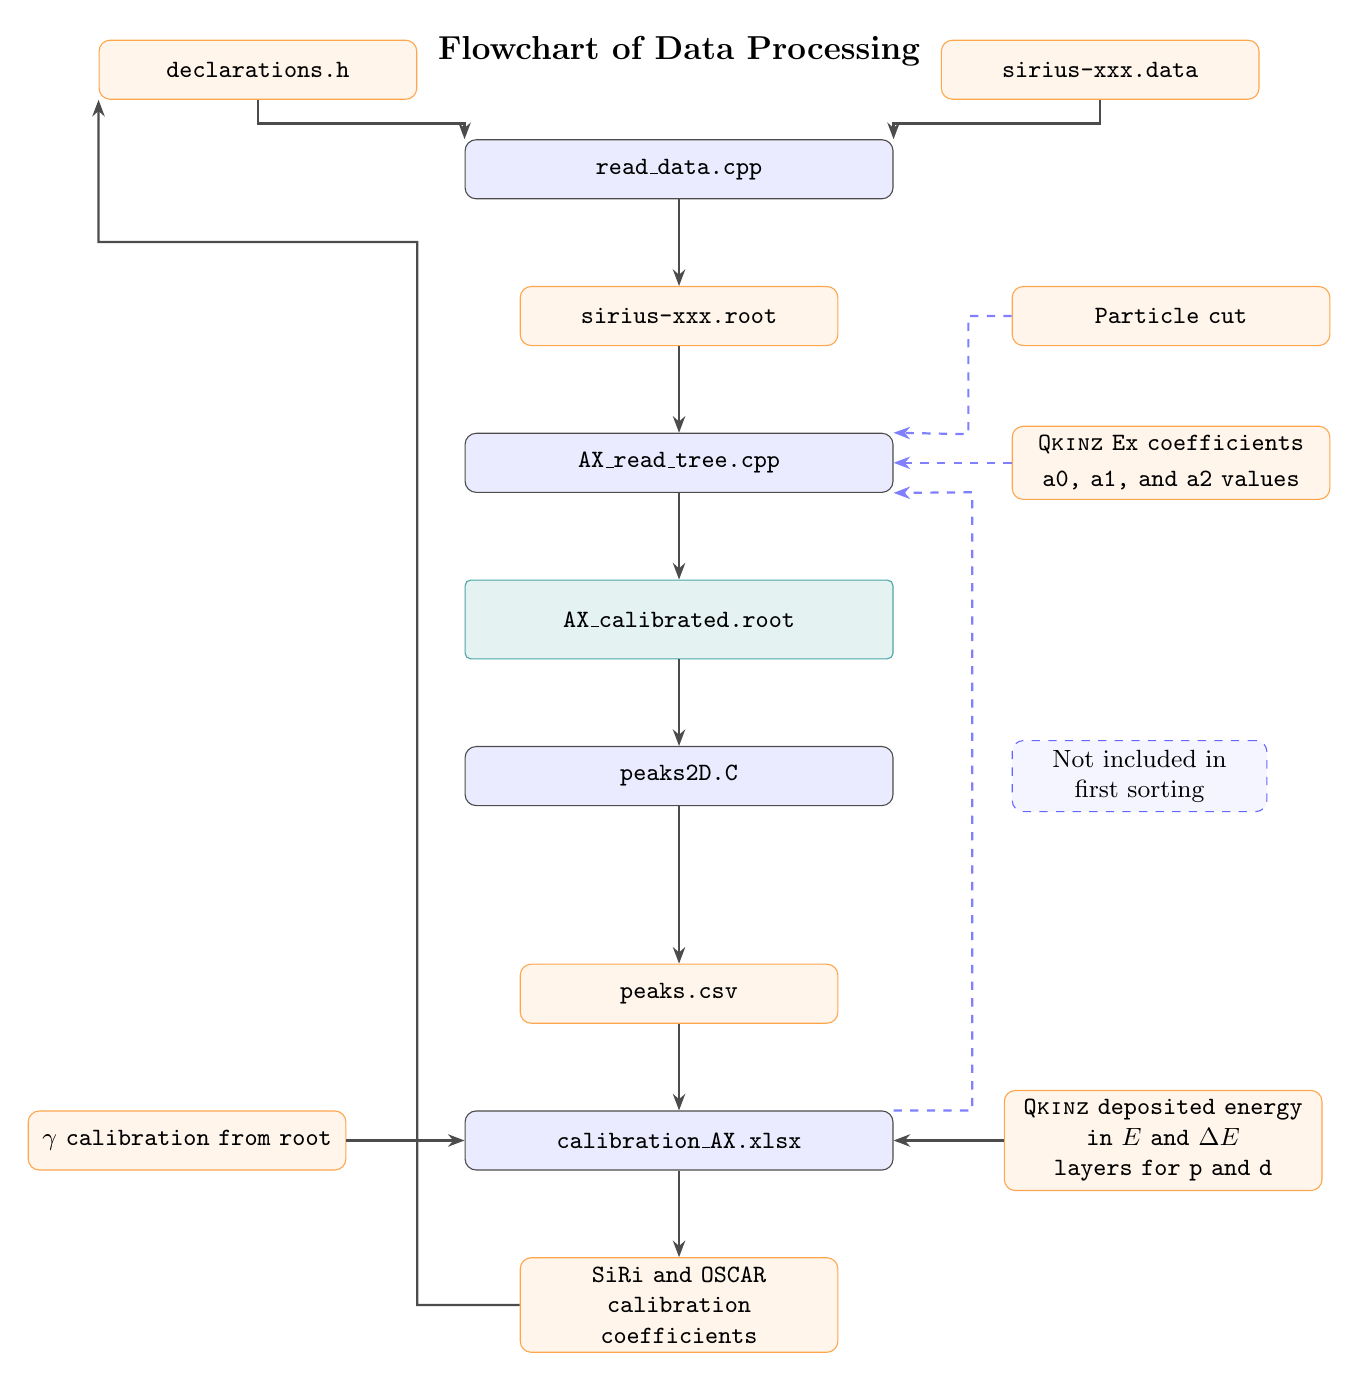
\begin{tikzpicture}[node distance=1.1cm and 2.4cm]

  % ── Title ──────────────────────────────────────────────────────────────────
  \node[font=\large\bfseries] (title) {Flowchart of Data Processing};

  % ── Main vertical chain ────────────────────────────────────────────────────
  \node[proc, below=0.8cm of title]
        (readdata)    {\texttt{read\_data.cpp}};

  \node[side, below=of readdata]
        (siriusroot)  {\texttt{sirius-xxx.root}};

  \node[proc, below=of siriusroot]
        (readtree)    {\texttt{AX\_read\_tree.cpp}};

  \node[file, below=of readtree]
        (calroot)     {\texttt{AX\_calibrated.root}};

  \node[proc, below=of calroot]
        (peaks2d)     {\texttt{peaks2D.C}};
  \node[side, below=2.0cm of peaks2d]
        (peakscsv)    {\texttt{peaks.csv}};

  \node[proc, below=of peakscsv]
        (calxlsx)     {\texttt{calibration\_AX.xlsx}};

  \node[side, right=1.4cm of calxlsx]
        (qkinz)       {Q\textsc{kinz} deposited energy\\
        in $E$ and $\Delta E$ layers for p and d};
        
  \node[side, below=of calxlsx]
        (siricoeff)   {SiRi and OSCAR calibration coefficients};

  \node[opt, right=1.5cm of peaks2d]
        (optexplaination) {Not included in \\
        first sorting};

  % ── NEW: gamma calibration branch (right side of calroot) ──────────────────
  \node[side, left=1.5cm of calxlsx]
        (gammacal)    {$\gamma$ calibration from root};

  % ── Input nodes (top) ──────────────────────────────────────────────────────
  \node[side, above left=0.5cm and 0.6cm of readdata]
        (declhin)     {\texttt{declarations.h}};
  \node[side, above right=0.5cm and 0.6cm of readdata]
        (siriusdata)  {\texttt{sirius-xxx.data}};

  % ── Feedback loop (drawn early so nodes render on top) ─────────────────────
  \draw[arr] (siricoeff.west)
             -- ++(-1.3,0)
             -- ++(0, 13.5)
             -- ++(-4.05,0)
             -- (declhin.south west);

  % ── Side output: peaks.csv ─────────────────────────────────────────────────

  % ── Side input to Qkinz ────────────────────────────────────────────────────
  \node[side, right = 2.2cm of siriusroot]
        (protoncut) {Particle cut};
  
  \node[side, right=1.5cm of readtree]
        (excoeff)     {%
          \textsc{Qkinz} Ex coefficients\\[2pt]
          a0, a1, and a2 values};

  % ── OPTIONAL box ───────────────────────────────────────────────────────────
  % \node[opt, right=2.0cm of readtree, yshift=0.2cm]
  %       (optional)    {%
  %         \textbf{\textsc{Calculated}}\\[3pt]
  %         $E\Delta E$ calibration coeffs.\\[2pt]
  %         $\gamma$ calibration coefficients};

  % ── Arrows: main chain ─────────────────────────────────────────────────────
  \draw[arr] (declhin.south)    -- ++(0,-0.3) -| (readdata.north west);
  \draw[arr] (siriusdata.south) -- ++(0,-0.3) -| (readdata.north east);

  \draw[arr] (readdata)   -- (siriusroot);
  \draw[arr] (siriusroot) -- (readtree);
  \draw[arr] (readtree)   -- (calroot);
  \draw[arr] (calroot)    -- (peaks2d);

  % % Direct arrow: peaks2D.C → calxlsx (left side, offset to avoid overlap)
  % \draw[arr] (peaks2d.west) -- ++(-0.6,0) -- ++(0,-3.3) -| (calxlsx.west);

  \draw[arr] (qkinz)      -- (calxlsx);
  \draw[arr] (calxlsx)    -- (siricoeff);

  % ── gamma calibration chain ────────────────────────────────────────────────
  % \draw[arr] (calroot.east) -- (gammacal.west);
  \draw[arr] (gammacal.east) --(calxlsx);

  % ── Arrows: side branches ──────────────────────────────────────────────────
  % peaks.csv side output (kept for reference, but direct arrow added above)
  \draw[arr] (peaks2d) -- (peakscsv);
  \draw[arr] (peakscsv) --  (calxlsx);

  % \draw[arr] (excoeff.west)  -- ++(-1,0)   -- (calxlsx.east);
  \draw[darr] (protoncut.west) -- ++(-0.55, 0) -- ++(0,-1.50) -- (readtree.north east);
  \draw[darr] (excoeff.west)  -- (readtree.east);
  % \draw[darr] (optional.west) -- (readtree.east);
  \draw[darr] (calxlsx.north east) -- ++(1,0) -- ++(0,7.85) -- (readtree.south east);

\end{tikzpicture}
\end{document}